\subsection{Аналитический способ.}
\subsubsection{С помощью формулы Грина.}
\begin{center}
    
Теорема грина гласит, что для функций $P,Q \in C^1(\text{cl}D)$.

$$\ointctrclockwise_{L} P \, dx + Q \, dy = \iint_{D} \left( \dfrac{\partial Q}{\partial x} - \dfrac{\partial P}{\partial y} \right)\,dx\,dy$$

В нашем случае, $P=xy^2, Q=-x^2y. \quad P,Q \in C^1(\mathbb{R})$

$$\dfrac{\partial Q}{\partial x} = \dfrac{\partial}{\partial x}\left(-x^2y\right) = -2xy \quad\quad \dfrac{\partial P}{\partial y} = \dfrac{\partial}{\partial y}\left(xy^2\right) = 2xy $$

Теперь нужно поменять знак двойного интеграла, потому что мы идем в отрицательном направлении.

$$ \varointclockwise_L xy^2 \,dx - x^2y \,dy = - \iint_D (-2xy - 2xy)\,dx\,dy = \iint_D 4xy \,dx\,dy = 4\iint_D xy \,dx\,dy$$

Перейдем в полярные координаты. 

$$
\begin{cases}
    x^2+y^2 \leq 16 = 4^2\\
    x+y\leq0
\end{cases} \Rightarrow\quad 
\begin{cases}
    x = r\cos{\phi}\\
    y = r\sin{\phi}\\
    r\in[0, 4]\\
    r\cos{\phi}+r\sin{\phi}\leq0
\end{cases} \Rightarrow\quad 
\cos{\phi}+\sin{\phi}\leq0 \Rightarrow\quad \phi\in\left[\dfrac{3\pi}{4}, \dfrac{7\pi}{4} \right]
$$

$$4\iint_D xy \,dx\,dy = \int_0^4 dr \int_{3\pi/4}^{7\pi/4} r^2\cos{\phi}\sin{\phi} \,d\phi = \dfrac{1}{2}\int_0^4 r^2\,dr\int_{3\pi/4}^{7\pi/4} \sin{2\phi} \,d\phi = $$
$$=\dfrac{1}{4}\int_0^4 r^2\,dr\int_{3\pi/4}^{7\pi/4} \sin{2\phi} \,d2\phi = \dfrac{1}{4}\int_0^4 r^2 \left[ \cos{2\phi} \right]_{3\pi/4}^{7\pi/4}  \,dr  = \dfrac{1}{4}\int_0^4 r^2 \left[ 0-0 \right]\,dr = \boxed{0} $$
\end{center}

\subsubsection{С помощью т. О вычислении КИ-2.}

$$\varointclockwise_L xy^2 \,dx - x^2y \,dy$$
\begin{center}
    
Пусть $\vv{F} = (F_1, F_2) = (xy^2, - x^2y), \quad d\vv{r} = (dx,dy), \quad \gamma(t): \mathbb{R} \rightarrow \mathbb{R}^2$ - путь по $L$.

$$\varointclockwise_L xy^2 \,dx - x^2y \,dy = \varointclockwise_L \vv{F} \cdot d\vv{r} = \int_a^b \left(F(\gamma(t))\cdot\gamma'(t)\right)dt$$

\begin{figure}[h!t]
    \centering
    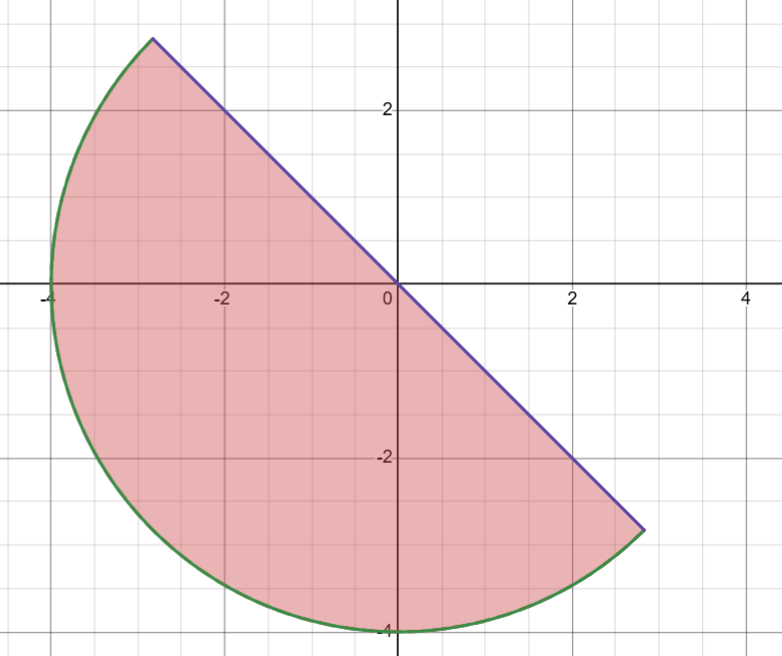
\includegraphics[width=0.75\linewidth]{Task10/Figure_D.png}
    \caption{Задание 10. Область D.}
    \label{task-10:figure-D}
\end{figure}

Разобьем кривую $L$ на две: $L_1$ и $L_2$ и присвоим им соответствующие пути $\gamma_1(t)$ и $\gamma_2(t)$. Пусть $\gamma_1$ проходит по прямой $y=-x$, на рисунке \ref{task-10:figure-D} он показан фиолетовым. Тогда $\gamma_2$ проходит по зеленой полуокружности, по часовой стрелке.
$$\gamma_1(t) = (t,-t), \quad t\in[-2\sqrt{2}, 2\sqrt{2}]$$
$$\gamma_2(t) = (4\sin{t}, 4\cos{t}), \quad t\in[3\pi/4, 7\pi/4]$$
$$\gamma_1'(t) = (1,-1), \quad \gamma_2'(t) = (4\cos{t}, -4\sin{t})$$


В $\gamma_2$ мы поменяли синус и косинус местами, чтобы он шел в правильном направлении, по часовой стрелке.

$$\varointclockwise_L \vv{F} \cdot d\vv{r} = \varointclockwise_{L_1} \vv{F} \cdot d\vv{r} + \varointclockwise_{L_2} \vv{F} \cdot d\vv{r} = \int_{-2\sqrt{2}}^{2\sqrt{2}} \left(F(\gamma_1(t))\cdot\gamma_1'(t)\right)dt + \int_{3\pi/4}^{7\pi/4} \left(F(\gamma_2(t))\cdot\gamma_2'(t)\right)dt = $$

$$= \int_{-2\sqrt{2}}^{2\sqrt{2}} \left((t(-t)^2, - t^2(-t)) \cdot (1,-1)) \right)\, dt +$$ 
$$+\int_{3\pi/4}^{7\pi/4} \left((4\sin{t})(4\cos{t})^2, - (4\sin{t})^2(4\cos{t}))\cdot(4\cos{t}, -4\sin{t})\right)\,dt = $$
$$= \int_{-2\sqrt{2}}^{2\sqrt{2}} t^3 - t^3\, dt + \int_{3\pi/4}^{7\pi/4} 256\sin{t}\cos^3{t} + 256\sin^3{t}\cos{t}\,dt =$$
$$= \int_{-2\sqrt{2}}^{2\sqrt{2}} 0\, dt + 256\int_{3\pi/4}^{7\pi/4} \sin{t}\cos{t}(\cos^2{t} + \sin^2{t})\,dt =256\int_{3\pi/4}^{7\pi/4} \sin{t}\cos{t}\,dt =$$
$$= 128\int_{3\pi/4}^{7\pi/4} \sin{2t}\,dt = 64\int_{3\pi/4}^{7\pi/4} \sin{2t}\,d2t = 64\left[ \cos{2\phi} \right]_{3\pi/4}^{7\pi/4} = 64[0-0]= \boxed{0}$$
\end{center}
